\documentclass[twoside]{book}

% Packages required by doxygen
\usepackage{fixltx2e}
\usepackage{calc}
\usepackage{doxygen}
\usepackage[export]{adjustbox} % also loads graphicx
\usepackage{graphicx}
\usepackage[utf8]{inputenc}
\usepackage{makeidx}
\usepackage{multicol}
\usepackage{multirow}
\PassOptionsToPackage{warn}{textcomp}
\usepackage{textcomp}
\usepackage[nointegrals]{wasysym}
\usepackage[table]{xcolor}

% Font selection
\usepackage[T1]{fontenc}
\usepackage[scaled=.90]{helvet}
\usepackage{courier}
\usepackage{amssymb}
\usepackage{sectsty}
\renewcommand{\familydefault}{\sfdefault}
\allsectionsfont{%
  \fontseries{bc}\selectfont%
  \color{darkgray}%
}
\renewcommand{\DoxyLabelFont}{%
  \fontseries{bc}\selectfont%
  \color{darkgray}%
}
\newcommand{\+}{\discretionary{\mbox{\scriptsize$\hookleftarrow$}}{}{}}

% Page & text layout
\usepackage{geometry}
\geometry{%
  a4paper,%
  top=2.5cm,%
  bottom=2.5cm,%
  left=2.5cm,%
  right=2.5cm%
}
\tolerance=750
\hfuzz=15pt
\hbadness=750
\setlength{\emergencystretch}{15pt}
\setlength{\parindent}{0cm}
\setlength{\parskip}{3ex plus 2ex minus 2ex}
\makeatletter
\renewcommand{\paragraph}{%
  \@startsection{paragraph}{4}{0ex}{-1.0ex}{1.0ex}{%
    \normalfont\normalsize\bfseries\SS@parafont%
  }%
}
\renewcommand{\subparagraph}{%
  \@startsection{subparagraph}{5}{0ex}{-1.0ex}{1.0ex}{%
    \normalfont\normalsize\bfseries\SS@subparafont%
  }%
}
\makeatother

% Headers & footers
\usepackage{fancyhdr}
\pagestyle{fancyplain}
\fancyhead[LE]{\fancyplain{}{\bfseries\thepage}}
\fancyhead[CE]{\fancyplain{}{}}
\fancyhead[RE]{\fancyplain{}{\bfseries\leftmark}}
\fancyhead[LO]{\fancyplain{}{\bfseries\rightmark}}
\fancyhead[CO]{\fancyplain{}{}}
\fancyhead[RO]{\fancyplain{}{\bfseries\thepage}}
\fancyfoot[LE]{\fancyplain{}{}}
\fancyfoot[CE]{\fancyplain{}{}}
\fancyfoot[RE]{\fancyplain{}{\bfseries\scriptsize Generated by Doxygen }}
\fancyfoot[LO]{\fancyplain{}{\bfseries\scriptsize Generated by Doxygen }}
\fancyfoot[CO]{\fancyplain{}{}}
\fancyfoot[RO]{\fancyplain{}{}}
\renewcommand{\footrulewidth}{0.4pt}
\renewcommand{\chaptermark}[1]{%
  \markboth{#1}{}%
}
\renewcommand{\sectionmark}[1]{%
  \markright{\thesection\ #1}%
}

% Indices & bibliography
\usepackage{natbib}
\usepackage[titles]{tocloft}
\setcounter{tocdepth}{3}
\setcounter{secnumdepth}{5}
\makeindex

% Hyperlinks (required, but should be loaded last)
\usepackage{ifpdf}
\ifpdf
  \usepackage[pdftex,pagebackref=true]{hyperref}
\else
  \usepackage[ps2pdf,pagebackref=true]{hyperref}
\fi
\hypersetup{%
  colorlinks=true,%
  linkcolor=blue,%
  citecolor=blue,%
  unicode%
}

% Custom commands
\newcommand{\clearemptydoublepage}{%
  \newpage{\pagestyle{empty}\cleardoublepage}%
}

\usepackage{caption}
\captionsetup{labelsep=space,justification=centering,font={bf},singlelinecheck=off,skip=4pt,position=top}

%===== C O N T E N T S =====

\begin{document}

% Titlepage & ToC
\hypersetup{pageanchor=false,
             bookmarksnumbered=true,
             pdfencoding=unicode
            }
\pagenumbering{alph}
\begin{titlepage}
\vspace*{7cm}
\begin{center}%
{\Large My Project }\\
\vspace*{1cm}
{\large Generated by Doxygen 1.8.13}\\
\end{center}
\end{titlepage}
\clearemptydoublepage
\pagenumbering{roman}
\tableofcontents
\clearemptydoublepage
\pagenumbering{arabic}
\hypersetup{pageanchor=true}

%--- Begin generated contents ---
\chapter{trabalho\+\_\+3\+\_\+metodos}
\label{md_README}
\Hypertarget{md_README}
\input{md_README}
\chapter{File Index}
\section{File List}
Here is a list of all files with brief descriptions\+:\begin{DoxyCompactList}
\item\contentsline{section}{\hyperlink{first__program_8cpp}{first\+\_\+program.\+cpp} }{\pageref{first__program_8cpp}}{}
\item\contentsline{section}{\hyperlink{leitor__arquivo_8cpp}{leitor\+\_\+arquivo.\+cpp} }{\pageref{leitor__arquivo_8cpp}}{}
\item\contentsline{section}{\hyperlink{main_8cpp}{main.\+cpp} }{\pageref{main_8cpp}}{}
\end{DoxyCompactList}

\chapter{File Documentation}
\hypertarget{first__program_8cpp}{}\section{first\+\_\+program.\+cpp File Reference}
\label{first__program_8cpp}\index{first\+\_\+program.\+cpp@{first\+\_\+program.\+cpp}}
{\ttfamily \#include $<$iostream$>$}\newline
Include dependency graph for first\+\_\+program.\+cpp\+:
\nopagebreak
\begin{figure}[H]
\begin{center}
\leavevmode
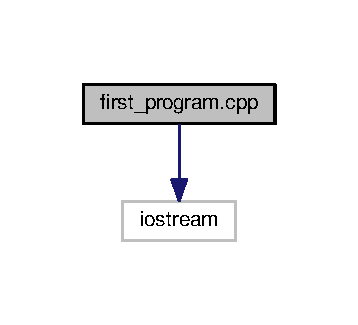
\includegraphics[width=172pt]{first__program_8cpp__incl}
\end{center}
\end{figure}
\subsection*{Functions}
\begin{DoxyCompactItemize}
\item 
int \hyperlink{first__program_8cpp_abf9e6b7e6f15df4b525a2e7705ba3089}{main} (int argc, char const $\ast$argv\mbox{[}$\,$\mbox{]})
\end{DoxyCompactItemize}


\subsection{Function Documentation}
\mbox{\Hypertarget{first__program_8cpp_abf9e6b7e6f15df4b525a2e7705ba3089}\label{first__program_8cpp_abf9e6b7e6f15df4b525a2e7705ba3089}} 
\index{first\+\_\+program.\+cpp@{first\+\_\+program.\+cpp}!main@{main}}
\index{main@{main}!first\+\_\+program.\+cpp@{first\+\_\+program.\+cpp}}
\subsubsection{\texorpdfstring{main()}{main()}}
{\footnotesize\ttfamily int main (\begin{DoxyParamCaption}\item[{int}]{argc,  }\item[{char const $\ast$}]{argv\mbox{[}$\,$\mbox{]} }\end{DoxyParamCaption})}


\hypertarget{leitor__arquivo_8cpp}{}\section{leitor\+\_\+arquivo.\+cpp File Reference}
\label{leitor__arquivo_8cpp}\index{leitor\+\_\+arquivo.\+cpp@{leitor\+\_\+arquivo.\+cpp}}
{\ttfamily \#include $<$iostream$>$}\newline
{\ttfamily \#include $<$boost/algorithm/string.\+hpp$>$}\newline
{\ttfamily \#include \char`\"{}leitor\+\_\+arquivo.\+hpp\char`\"{}}\newline
Include dependency graph for leitor\+\_\+arquivo.\+cpp\+:
\nopagebreak
\begin{figure}[H]
\begin{center}
\leavevmode
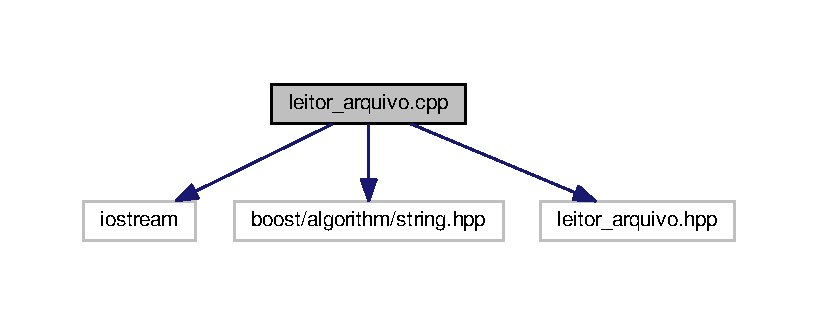
\includegraphics[width=350pt]{leitor__arquivo_8cpp__incl}
\end{center}
\end{figure}
\subsection*{Functions}
\begin{DoxyCompactItemize}
\item 
int \hyperlink{leitor__arquivo_8cpp_ac7fd2c9d88aee5243a02876ff6160187}{verifica\+Arquivo} (fstream $\ast$arquivo\+Prog, string arquivo\+Str)
\item 
int \hyperlink{leitor__arquivo_8cpp_a67a02f1d485e8c536a115a8509badc14}{verifica\+Linhas} (fstream $\ast$arquivo\+Prog, int \&pos\+Linha)
\item 
int \hyperlink{leitor__arquivo_8cpp_a5913852cf583808d86998bfa41db3221}{contagem\+Branco\+Comentario} (fstream $\ast$arquivo\+Prog, int \&pos\+Linha)
\end{DoxyCompactItemize}


\subsection{Function Documentation}
\mbox{\Hypertarget{leitor__arquivo_8cpp_a5913852cf583808d86998bfa41db3221}\label{leitor__arquivo_8cpp_a5913852cf583808d86998bfa41db3221}} 
\index{leitor\+\_\+arquivo.\+cpp@{leitor\+\_\+arquivo.\+cpp}!contagem\+Branco\+Comentario@{contagem\+Branco\+Comentario}}
\index{contagem\+Branco\+Comentario@{contagem\+Branco\+Comentario}!leitor\+\_\+arquivo.\+cpp@{leitor\+\_\+arquivo.\+cpp}}
\subsubsection{\texorpdfstring{contagem\+Branco\+Comentario()}{contagemBrancoComentario()}}
{\footnotesize\ttfamily int contagem\+Branco\+Comentario (\begin{DoxyParamCaption}\item[{fstream $\ast$}]{arquivo\+Prog,  }\item[{int \&}]{pos\+Linha }\end{DoxyParamCaption})}

\mbox{\Hypertarget{leitor__arquivo_8cpp_ac7fd2c9d88aee5243a02876ff6160187}\label{leitor__arquivo_8cpp_ac7fd2c9d88aee5243a02876ff6160187}} 
\index{leitor\+\_\+arquivo.\+cpp@{leitor\+\_\+arquivo.\+cpp}!verifica\+Arquivo@{verifica\+Arquivo}}
\index{verifica\+Arquivo@{verifica\+Arquivo}!leitor\+\_\+arquivo.\+cpp@{leitor\+\_\+arquivo.\+cpp}}
\subsubsection{\texorpdfstring{verifica\+Arquivo()}{verificaArquivo()}}
{\footnotesize\ttfamily int verifica\+Arquivo (\begin{DoxyParamCaption}\item[{fstream $\ast$}]{arquivo\+Prog,  }\item[{string}]{arquivo\+Str }\end{DoxyParamCaption})}

\mbox{\Hypertarget{leitor__arquivo_8cpp_a67a02f1d485e8c536a115a8509badc14}\label{leitor__arquivo_8cpp_a67a02f1d485e8c536a115a8509badc14}} 
\index{leitor\+\_\+arquivo.\+cpp@{leitor\+\_\+arquivo.\+cpp}!verifica\+Linhas@{verifica\+Linhas}}
\index{verifica\+Linhas@{verifica\+Linhas}!leitor\+\_\+arquivo.\+cpp@{leitor\+\_\+arquivo.\+cpp}}
\subsubsection{\texorpdfstring{verifica\+Linhas()}{verificaLinhas()}}
{\footnotesize\ttfamily int verifica\+Linhas (\begin{DoxyParamCaption}\item[{fstream $\ast$}]{arquivo\+Prog,  }\item[{int \&}]{pos\+Linha }\end{DoxyParamCaption})}


\hypertarget{main_8cpp}{}\section{main.\+cpp File Reference}
\label{main_8cpp}\index{main.\+cpp@{main.\+cpp}}
{\ttfamily \#include $<$iostream$>$}\newline
{\ttfamily \#include \char`\"{}leitor\+\_\+arquivo.\+hpp\char`\"{}}\newline
Include dependency graph for main.\+cpp\+:
\nopagebreak
\begin{figure}[H]
\begin{center}
\leavevmode
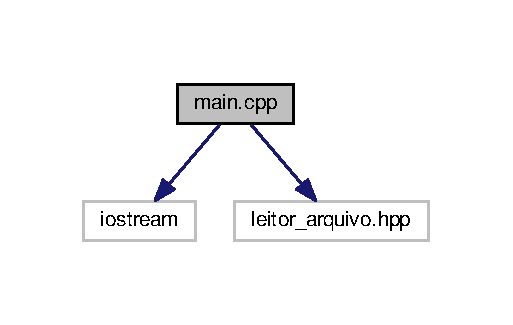
\includegraphics[width=246pt]{main_8cpp__incl}
\end{center}
\end{figure}
\subsection*{Functions}
\begin{DoxyCompactItemize}
\item 
int \hyperlink{main_8cpp_abf9e6b7e6f15df4b525a2e7705ba3089}{main} (int argc, char const $\ast$argv\mbox{[}$\,$\mbox{]})
\begin{DoxyCompactList}\small\item\em Programa principal. \end{DoxyCompactList}\end{DoxyCompactItemize}


\subsection{Function Documentation}
\mbox{\Hypertarget{main_8cpp_abf9e6b7e6f15df4b525a2e7705ba3089}\label{main_8cpp_abf9e6b7e6f15df4b525a2e7705ba3089}} 
\index{main.\+cpp@{main.\+cpp}!main@{main}}
\index{main@{main}!main.\+cpp@{main.\+cpp}}
\subsubsection{\texorpdfstring{main()}{main()}}
{\footnotesize\ttfamily int main (\begin{DoxyParamCaption}\item[{int}]{argc,  }\item[{char const $\ast$}]{argv\mbox{[}$\,$\mbox{]} }\end{DoxyParamCaption})}



Programa principal. 


\begin{DoxyParams}{Parameters}
{\em argc} & \\
\hline
{\em argv} & \\
\hline
\end{DoxyParams}
\begin{DoxyReturn}{Returns}
int 
\end{DoxyReturn}

\hypertarget{README_8md}{}\section{R\+E\+A\+D\+M\+E.\+md File Reference}
\label{README_8md}\index{R\+E\+A\+D\+M\+E.\+md@{R\+E\+A\+D\+M\+E.\+md}}

%--- End generated contents ---

% Index
\backmatter
\newpage
\phantomsection
\clearemptydoublepage
\addcontentsline{toc}{chapter}{Index}
\printindex

\end{document}
